%% \FloatBarrier
%% \subsection{Map service time} 

%% \begin{lstlisting}[morekeywords={servicet_stop, servicet_start, servicet_sum}]
%% void * generator_task(void *args...) {
%%   ...
%%   pthread_barrier_wait(...);
%%   for (i=0; i<m; i++) {
%%     a = get_clock_cycle();
%%     sym_send(ch_out, A_set[i]);
%%     while (get_clock_cycle() - a < Ta) 
%%       ;
%%   }
%%   ...
%% }

%% void * worker_task(void *args...) {
%%   ...
%%   servicet_stop = 0;
%%   pthread_barrier_wait(...);
%%   for (i=0; i<m; i++) {
%%     A = (int *)sym_receive(ch_in);
%%     atomic_compiler_barrier(); 
%%     if (rank == 0) {
%%       servicet_start = servicet_stop;
%%       servicet_stop = get_clock_cycle();
%%       if (servicet_start != 0)
%%         servicet_sum += servicet_stop - servicet_start;
%%     }
%%     atomic_compiler_barrier(); 
%%     if (ch_left != NULL) sym_send(ch_left, A);
%%     if (ch_right != NULL) sym_send(ch_right, A);
%%     for (j=0; j<g; j++) {
%%       C[j*rank] = 0;
%%       for (k=0; k<M; k++) 
%%         C[j*rank] = *(A+j*M+k) * B[k] + C[j*rank];
%%     }
%%     asymin_send(ch_out, C);
%%   }
%%   if (rank == 0)
%%     fprintf(output_file, ``%d %f\n'', n, (double)servicet_sum/m);
%%   ...
%% }

%% void * collector_task(void *args...) {
%%   ...
%%   pthread_barrier_wait(...);
%%   for (i=0; i<m; i++) {
%%     (void)asymin_receive(ch_in);
%%   }
%%   ...
%% }
%% \end{lstlisting}


\begin{figure}[p]
  \caption{Grafici di scalabilit\`a del tempo di servizio dello stream al variare del tempo di interarrivo}
  \begin{subfigure}[b]{.5\columnwidth}
    \centering
    \renewcommand\thesubfigure{\alph{subfigure}}
    %% se vuoi spostare questa caption in fondo devi modificare anche i contatori!
    \caption{Implementazione con solo UDN}
    \begin{subfigure}[b]{\textwidth}
      \centering
      \addtocounter{subfigure}{-1}
      \renewcommand\thesubfigure{\alph{subfigure}1}
      \resizebox{\columnwidth}{!}{% GNUPLOT: LaTeX picture with Postscript
\begingroup
  \makeatletter
  \providecommand\color[2][]{%
    \GenericError{(gnuplot) \space\space\space\@spaces}{%
      Package color not loaded in conjunction with
      terminal option `colourtext'%
    }{See the gnuplot documentation for explanation.%
    }{Either use 'blacktext' in gnuplot or load the package
      color.sty in LaTeX.}%
    \renewcommand\color[2][]{}%
  }%
  \providecommand\includegraphics[2][]{%
    \GenericError{(gnuplot) \space\space\space\@spaces}{%
      Package graphicx or graphics not loaded%
    }{See the gnuplot documentation for explanation.%
    }{The gnuplot epslatex terminal needs graphicx.sty or graphics.sty.}%
    \renewcommand\includegraphics[2][]{}%
  }%
  \providecommand\rotatebox[2]{#2}%
  \@ifundefined{ifGPcolor}{%
    \newif\ifGPcolor
    \GPcolortrue
  }{}%
  \@ifundefined{ifGPblacktext}{%
    \newif\ifGPblacktext
    \GPblacktexttrue
  }{}%
  % define a \g@addto@macro without @ in the name:
  \let\gplgaddtomacro\g@addto@macro
  % define empty templates for all commands taking text:
  \gdef\gplbacktext{}%
  \gdef\gplfronttext{}%
  \makeatother
  \ifGPblacktext
    % no textcolor at all
    \def\colorrgb#1{}%
    \def\colorgray#1{}%
  \else
    % gray or color?
    \ifGPcolor
      \def\colorrgb#1{\color[rgb]{#1}}%
      \def\colorgray#1{\color[gray]{#1}}%
      \expandafter\def\csname LTw\endcsname{\color{white}}%
      \expandafter\def\csname LTb\endcsname{\color{black}}%
      \expandafter\def\csname LTa\endcsname{\color{black}}%
      \expandafter\def\csname LT0\endcsname{\color[rgb]{1,0,0}}%
      \expandafter\def\csname LT1\endcsname{\color[rgb]{0,1,0}}%
      \expandafter\def\csname LT2\endcsname{\color[rgb]{0,0,1}}%
      \expandafter\def\csname LT3\endcsname{\color[rgb]{1,0,1}}%
      \expandafter\def\csname LT4\endcsname{\color[rgb]{0,1,1}}%
      \expandafter\def\csname LT5\endcsname{\color[rgb]{1,1,0}}%
      \expandafter\def\csname LT6\endcsname{\color[rgb]{0,0,0}}%
      \expandafter\def\csname LT7\endcsname{\color[rgb]{1,0.3,0}}%
      \expandafter\def\csname LT8\endcsname{\color[rgb]{0.5,0.5,0.5}}%
    \else
      % gray
      \def\colorrgb#1{\color{black}}%
      \def\colorgray#1{\color[gray]{#1}}%
      \expandafter\def\csname LTw\endcsname{\color{white}}%
      \expandafter\def\csname LTb\endcsname{\color{black}}%
      \expandafter\def\csname LTa\endcsname{\color{black}}%
      \expandafter\def\csname LT0\endcsname{\color{black}}%
      \expandafter\def\csname LT1\endcsname{\color{black}}%
      \expandafter\def\csname LT2\endcsname{\color{black}}%
      \expandafter\def\csname LT3\endcsname{\color{black}}%
      \expandafter\def\csname LT4\endcsname{\color{black}}%
      \expandafter\def\csname LT5\endcsname{\color{black}}%
      \expandafter\def\csname LT6\endcsname{\color{black}}%
      \expandafter\def\csname LT7\endcsname{\color{black}}%
      \expandafter\def\csname LT8\endcsname{\color{black}}%
    \fi
  \fi
  \setlength{\unitlength}{0.0500bp}%
  \begin{picture}(7200.00,5040.00)%
    \gplgaddtomacro\gplbacktext{%
      \csname LTb\endcsname%
      \put(814,1325){\makebox(0,0)[r]{\strut{} 10}}%
      \csname LTb\endcsname%
      \put(814,2015){\makebox(0,0)[r]{\strut{} 20}}%
      \csname LTb\endcsname%
      \put(814,2705){\makebox(0,0)[r]{\strut{} 30}}%
      \csname LTb\endcsname%
      \put(814,3395){\makebox(0,0)[r]{\strut{} 40}}%
      \csname LTb\endcsname%
      \put(814,4085){\makebox(0,0)[r]{\strut{} 50}}%
      \csname LTb\endcsname%
      \put(814,4775){\makebox(0,0)[r]{\strut{} 60}}%
      \csname LTb\endcsname%
      \put(1839,484){\makebox(0,0){\strut{} 10}}%
      \csname LTb\endcsname%
      \put(2832,484){\makebox(0,0){\strut{} 20}}%
      \csname LTb\endcsname%
      \put(3825,484){\makebox(0,0){\strut{} 30}}%
      \csname LTb\endcsname%
      \put(4818,484){\makebox(0,0){\strut{} 40}}%
      \csname LTb\endcsname%
      \put(5810,484){\makebox(0,0){\strut{} 50}}%
      \csname LTb\endcsname%
      \put(6803,484){\makebox(0,0){\strut{} 60}}%
      \put(176,2739){\rotatebox{-270}{\makebox(0,0){\strut{}scalability}}}%
      \put(3874,154){\makebox(0,0){\strut{}$n$ parallel degree}}%
    }%
    \gplgaddtomacro\gplfronttext{%
      \csname LTb\endcsname%
      \put(3322,4602){\makebox(0,0)[r]{\strut{}ideal scalability}}%
      \csname LTb\endcsname%
      \put(3322,4382){\makebox(0,0)[r]{\strut{}$T_A$ 20000 $\tau$}}%
      \csname LTb\endcsname%
      \put(3322,4162){\makebox(0,0)[r]{\strut{}$T_A$ 10000 $\tau$}}%
      \csname LTb\endcsname%
      \put(3322,3942){\makebox(0,0)[r]{\strut{}$T_A$ 7000 $\tau$}}%
      \csname LTb\endcsname%
      \put(3322,3722){\makebox(0,0)[r]{\strut{}$T_A$ 4000 $\tau$}}%
    }%
    \gplbacktext
    \put(0,0){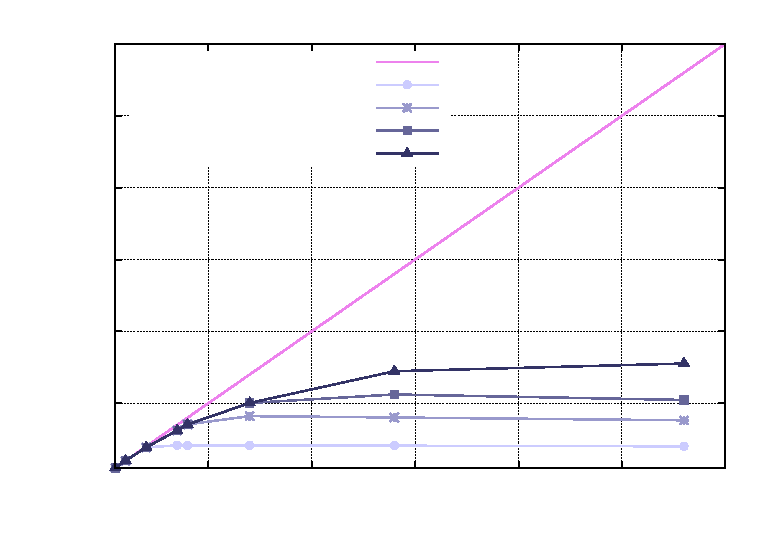
\includegraphics{plot-T-s_nogatherInt_00_500_selected_56}}%
    \gplfronttext
  \end{picture}%
\endgroup
}
      \caption{Scalabilit\`a dell'implementazione UDN con M=56 al variare del tempo di interarrivo}
      \label{fig:scalability_UDN_size56}
    \end{subfigure}
    ~
    \begin{subfigure}[b]{\textwidth}
      \centering
      \addtocounter{subfigure}{-1}
      \renewcommand\thesubfigure{\alph{subfigure}2}
      \resizebox{\columnwidth}{!}{% GNUPLOT: LaTeX picture with Postscript
\begingroup
  \makeatletter
  \providecommand\color[2][]{%
    \GenericError{(gnuplot) \space\space\space\@spaces}{%
      Package color not loaded in conjunction with
      terminal option `colourtext'%
    }{See the gnuplot documentation for explanation.%
    }{Either use 'blacktext' in gnuplot or load the package
      color.sty in LaTeX.}%
    \renewcommand\color[2][]{}%
  }%
  \providecommand\includegraphics[2][]{%
    \GenericError{(gnuplot) \space\space\space\@spaces}{%
      Package graphicx or graphics not loaded%
    }{See the gnuplot documentation for explanation.%
    }{The gnuplot epslatex terminal needs graphicx.sty or graphics.sty.}%
    \renewcommand\includegraphics[2][]{}%
  }%
  \providecommand\rotatebox[2]{#2}%
  \@ifundefined{ifGPcolor}{%
    \newif\ifGPcolor
    \GPcolortrue
  }{}%
  \@ifundefined{ifGPblacktext}{%
    \newif\ifGPblacktext
    \GPblacktexttrue
  }{}%
  % define a \g@addto@macro without @ in the name:
  \let\gplgaddtomacro\g@addto@macro
  % define empty templates for all commands taking text:
  \gdef\gplbacktext{}%
  \gdef\gplfronttext{}%
  \makeatother
  \ifGPblacktext
    % no textcolor at all
    \def\colorrgb#1{}%
    \def\colorgray#1{}%
  \else
    % gray or color?
    \ifGPcolor
      \def\colorrgb#1{\color[rgb]{#1}}%
      \def\colorgray#1{\color[gray]{#1}}%
      \expandafter\def\csname LTw\endcsname{\color{white}}%
      \expandafter\def\csname LTb\endcsname{\color{black}}%
      \expandafter\def\csname LTa\endcsname{\color{black}}%
      \expandafter\def\csname LT0\endcsname{\color[rgb]{1,0,0}}%
      \expandafter\def\csname LT1\endcsname{\color[rgb]{0,1,0}}%
      \expandafter\def\csname LT2\endcsname{\color[rgb]{0,0,1}}%
      \expandafter\def\csname LT3\endcsname{\color[rgb]{1,0,1}}%
      \expandafter\def\csname LT4\endcsname{\color[rgb]{0,1,1}}%
      \expandafter\def\csname LT5\endcsname{\color[rgb]{1,1,0}}%
      \expandafter\def\csname LT6\endcsname{\color[rgb]{0,0,0}}%
      \expandafter\def\csname LT7\endcsname{\color[rgb]{1,0.3,0}}%
      \expandafter\def\csname LT8\endcsname{\color[rgb]{0.5,0.5,0.5}}%
    \else
      % gray
      \def\colorrgb#1{\color{black}}%
      \def\colorgray#1{\color[gray]{#1}}%
      \expandafter\def\csname LTw\endcsname{\color{white}}%
      \expandafter\def\csname LTb\endcsname{\color{black}}%
      \expandafter\def\csname LTa\endcsname{\color{black}}%
      \expandafter\def\csname LT0\endcsname{\color{black}}%
      \expandafter\def\csname LT1\endcsname{\color{black}}%
      \expandafter\def\csname LT2\endcsname{\color{black}}%
      \expandafter\def\csname LT3\endcsname{\color{black}}%
      \expandafter\def\csname LT4\endcsname{\color{black}}%
      \expandafter\def\csname LT5\endcsname{\color{black}}%
      \expandafter\def\csname LT6\endcsname{\color{black}}%
      \expandafter\def\csname LT7\endcsname{\color{black}}%
      \expandafter\def\csname LT8\endcsname{\color{black}}%
    \fi
  \fi
  \setlength{\unitlength}{0.0500bp}%
  \begin{picture}(7200.00,5040.00)%
    \gplgaddtomacro\gplbacktext{%
      \csname LTb\endcsname%
      \put(814,1325){\makebox(0,0)[r]{\strut{} 10}}%
      \csname LTb\endcsname%
      \put(814,2015){\makebox(0,0)[r]{\strut{} 20}}%
      \csname LTb\endcsname%
      \put(814,2705){\makebox(0,0)[r]{\strut{} 30}}%
      \csname LTb\endcsname%
      \put(814,3395){\makebox(0,0)[r]{\strut{} 40}}%
      \csname LTb\endcsname%
      \put(814,4085){\makebox(0,0)[r]{\strut{} 50}}%
      \csname LTb\endcsname%
      \put(814,4775){\makebox(0,0)[r]{\strut{} 60}}%
      \csname LTb\endcsname%
      \put(1839,484){\makebox(0,0){\strut{} 10}}%
      \csname LTb\endcsname%
      \put(2832,484){\makebox(0,0){\strut{} 20}}%
      \csname LTb\endcsname%
      \put(3825,484){\makebox(0,0){\strut{} 30}}%
      \csname LTb\endcsname%
      \put(4818,484){\makebox(0,0){\strut{} 40}}%
      \csname LTb\endcsname%
      \put(5810,484){\makebox(0,0){\strut{} 50}}%
      \csname LTb\endcsname%
      \put(6803,484){\makebox(0,0){\strut{} 60}}%
      \put(176,2739){\rotatebox{-270}{\makebox(0,0){\strut{}scalability}}}%
      \put(3874,154){\makebox(0,0){\strut{}$n$ parallel degree}}%
    }%
    \gplgaddtomacro\gplfronttext{%
      \csname LTb\endcsname%
      \put(3322,4602){\makebox(0,0)[r]{\strut{}ideal scalability}}%
      \csname LTb\endcsname%
      \put(3322,4382){\makebox(0,0)[r]{\strut{}$T_A$ 150000 $\tau$}}%
      \csname LTb\endcsname%
      \put(3322,4162){\makebox(0,0)[r]{\strut{}$T_A$ 80000 $\tau$}}%
      \csname LTb\endcsname%
      \put(3322,3942){\makebox(0,0)[r]{\strut{}$T_A$ 50000 $\tau$}}%
      \csname LTb\endcsname%
      \put(3322,3722){\makebox(0,0)[r]{\strut{}$T_A$ 35000 $\tau$}}%
      \csname LTb\endcsname%
      \put(3322,3502){\makebox(0,0)[r]{\strut{}$T_A$ 20000 $\tau$}}%
    }%
    \gplbacktext
    \put(0,0){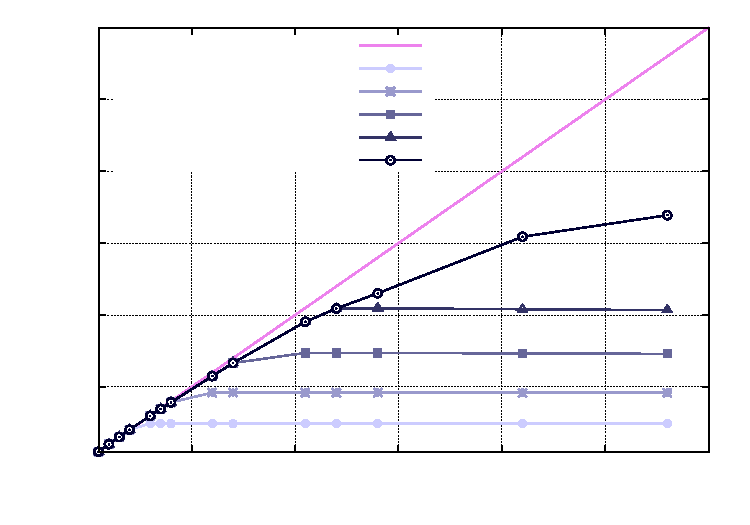
\includegraphics{plot-T-s_nogatherInt_00_500_selected_168}}%
    \gplfronttext
  \end{picture}%
\endgroup
}
      \caption{Scalabilit\`a dell'implementazione UDN con M=168 al variare del tempo di interarrivo}
      \label{fig:scalability_UDN_size168}
    \end{subfigure}
    ~
    \begin{subfigure}[b]{\textwidth}
      \centering
      \addtocounter{subfigure}{-1}
      \renewcommand\thesubfigure{\alph{subfigure}3}
      \resizebox{\columnwidth}{!}{% GNUPLOT: LaTeX picture with Postscript
\begingroup
  \makeatletter
  \providecommand\color[2][]{%
    \GenericError{(gnuplot) \space\space\space\@spaces}{%
      Package color not loaded in conjunction with
      terminal option `colourtext'%
    }{See the gnuplot documentation for explanation.%
    }{Either use 'blacktext' in gnuplot or load the package
      color.sty in LaTeX.}%
    \renewcommand\color[2][]{}%
  }%
  \providecommand\includegraphics[2][]{%
    \GenericError{(gnuplot) \space\space\space\@spaces}{%
      Package graphicx or graphics not loaded%
    }{See the gnuplot documentation for explanation.%
    }{The gnuplot epslatex terminal needs graphicx.sty or graphics.sty.}%
    \renewcommand\includegraphics[2][]{}%
  }%
  \providecommand\rotatebox[2]{#2}%
  \@ifundefined{ifGPcolor}{%
    \newif\ifGPcolor
    \GPcolortrue
  }{}%
  \@ifundefined{ifGPblacktext}{%
    \newif\ifGPblacktext
    \GPblacktexttrue
  }{}%
  % define a \g@addto@macro without @ in the name:
  \let\gplgaddtomacro\g@addto@macro
  % define empty templates for all commands taking text:
  \gdef\gplbacktext{}%
  \gdef\gplfronttext{}%
  \makeatother
  \ifGPblacktext
    % no textcolor at all
    \def\colorrgb#1{}%
    \def\colorgray#1{}%
  \else
    % gray or color?
    \ifGPcolor
      \def\colorrgb#1{\color[rgb]{#1}}%
      \def\colorgray#1{\color[gray]{#1}}%
      \expandafter\def\csname LTw\endcsname{\color{white}}%
      \expandafter\def\csname LTb\endcsname{\color{black}}%
      \expandafter\def\csname LTa\endcsname{\color{black}}%
      \expandafter\def\csname LT0\endcsname{\color[rgb]{1,0,0}}%
      \expandafter\def\csname LT1\endcsname{\color[rgb]{0,1,0}}%
      \expandafter\def\csname LT2\endcsname{\color[rgb]{0,0,1}}%
      \expandafter\def\csname LT3\endcsname{\color[rgb]{1,0,1}}%
      \expandafter\def\csname LT4\endcsname{\color[rgb]{0,1,1}}%
      \expandafter\def\csname LT5\endcsname{\color[rgb]{1,1,0}}%
      \expandafter\def\csname LT6\endcsname{\color[rgb]{0,0,0}}%
      \expandafter\def\csname LT7\endcsname{\color[rgb]{1,0.3,0}}%
      \expandafter\def\csname LT8\endcsname{\color[rgb]{0.5,0.5,0.5}}%
    \else
      % gray
      \def\colorrgb#1{\color{black}}%
      \def\colorgray#1{\color[gray]{#1}}%
      \expandafter\def\csname LTw\endcsname{\color{white}}%
      \expandafter\def\csname LTb\endcsname{\color{black}}%
      \expandafter\def\csname LTa\endcsname{\color{black}}%
      \expandafter\def\csname LT0\endcsname{\color{black}}%
      \expandafter\def\csname LT1\endcsname{\color{black}}%
      \expandafter\def\csname LT2\endcsname{\color{black}}%
      \expandafter\def\csname LT3\endcsname{\color{black}}%
      \expandafter\def\csname LT4\endcsname{\color{black}}%
      \expandafter\def\csname LT5\endcsname{\color{black}}%
      \expandafter\def\csname LT6\endcsname{\color{black}}%
      \expandafter\def\csname LT7\endcsname{\color{black}}%
      \expandafter\def\csname LT8\endcsname{\color{black}}%
    \fi
  \fi
  \setlength{\unitlength}{0.0500bp}%
  \begin{picture}(7200.00,5040.00)%
    \gplgaddtomacro\gplbacktext{%
      \csname LTb\endcsname%
      \put(814,1325){\makebox(0,0)[r]{\strut{} 10}}%
      \csname LTb\endcsname%
      \put(814,2015){\makebox(0,0)[r]{\strut{} 20}}%
      \csname LTb\endcsname%
      \put(814,2705){\makebox(0,0)[r]{\strut{} 30}}%
      \csname LTb\endcsname%
      \put(814,3395){\makebox(0,0)[r]{\strut{} 40}}%
      \csname LTb\endcsname%
      \put(814,4085){\makebox(0,0)[r]{\strut{} 50}}%
      \csname LTb\endcsname%
      \put(814,4775){\makebox(0,0)[r]{\strut{} 60}}%
      \csname LTb\endcsname%
      \put(1839,484){\makebox(0,0){\strut{} 10}}%
      \csname LTb\endcsname%
      \put(2832,484){\makebox(0,0){\strut{} 20}}%
      \csname LTb\endcsname%
      \put(3825,484){\makebox(0,0){\strut{} 30}}%
      \csname LTb\endcsname%
      \put(4818,484){\makebox(0,0){\strut{} 40}}%
      \csname LTb\endcsname%
      \put(5810,484){\makebox(0,0){\strut{} 50}}%
      \csname LTb\endcsname%
      \put(6803,484){\makebox(0,0){\strut{} 60}}%
      \put(176,2739){\rotatebox{-270}{\makebox(0,0){\strut{}scalability}}}%
      \put(3874,154){\makebox(0,0){\strut{}$n$ parallel degree}}%
    }%
    \gplgaddtomacro\gplfronttext{%
      \csname LTb\endcsname%
      \put(3322,4602){\makebox(0,0)[r]{\strut{}ideal scalability}}%
      \csname LTb\endcsname%
      \put(3322,4382){\makebox(0,0)[r]{\strut{}$T_A$ 250000 $\tau$}}%
      \csname LTb\endcsname%
      \put(3322,4162){\makebox(0,0)[r]{\strut{}$T_A$ 150000 $\tau$}}%
      \csname LTb\endcsname%
      \put(3322,3942){\makebox(0,0)[r]{\strut{}$T_A$ 100000 $\tau$}}%
      \csname LTb\endcsname%
      \put(3322,3722){\makebox(0,0)[r]{\strut{}$T_A$ 80000 $\tau$}}%
      \csname LTb\endcsname%
      \put(3322,3502){\makebox(0,0)[r]{\strut{}$T_A$ 50000 $\tau$}}%
    }%
    \gplbacktext
    \put(0,0){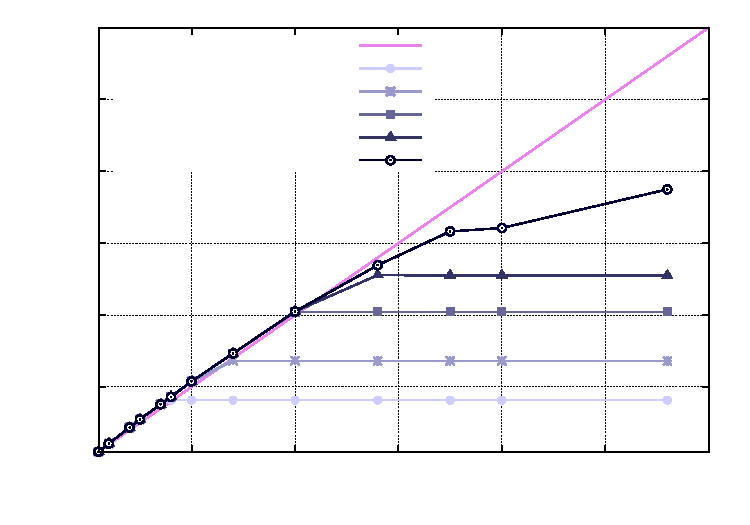
\includegraphics{plot-T-s_nogatherInt_00_500_selected_280}}%
    \gplfronttext
  \end{picture}%
\endgroup
}
      \caption{Scalabilit\`a dell'implementazione UDN con M=280 al variare del tempo di interarrivo}
      \label{fig:scalability_UDN_size280}
    \end{subfigure}
    \label{fig:allScalbility_UDN}
  \end{subfigure}
  \hspace{2ex}
  \begin{subfigure}[b]{.5\columnwidth}
    \centering
    \renewcommand\thesubfigure{\alph{subfigure}}
    \caption{Implementazione con solo SM}
    \begin{subfigure}[b]{\textwidth}
      \centering
      \addtocounter{subfigure}{-1}
      \renewcommand\thesubfigure{\alph{subfigure}1}
      \resizebox{\columnwidth}{!}{% GNUPLOT: LaTeX picture with Postscript
\begingroup
  \makeatletter
  \providecommand\color[2][]{%
    \GenericError{(gnuplot) \space\space\space\@spaces}{%
      Package color not loaded in conjunction with
      terminal option `colourtext'%
    }{See the gnuplot documentation for explanation.%
    }{Either use 'blacktext' in gnuplot or load the package
      color.sty in LaTeX.}%
    \renewcommand\color[2][]{}%
  }%
  \providecommand\includegraphics[2][]{%
    \GenericError{(gnuplot) \space\space\space\@spaces}{%
      Package graphicx or graphics not loaded%
    }{See the gnuplot documentation for explanation.%
    }{The gnuplot epslatex terminal needs graphicx.sty or graphics.sty.}%
    \renewcommand\includegraphics[2][]{}%
  }%
  \providecommand\rotatebox[2]{#2}%
  \@ifundefined{ifGPcolor}{%
    \newif\ifGPcolor
    \GPcolortrue
  }{}%
  \@ifundefined{ifGPblacktext}{%
    \newif\ifGPblacktext
    \GPblacktexttrue
  }{}%
  % define a \g@addto@macro without @ in the name:
  \let\gplgaddtomacro\g@addto@macro
  % define empty templates for all commands taking text:
  \gdef\gplbacktext{}%
  \gdef\gplfronttext{}%
  \makeatother
  \ifGPblacktext
    % no textcolor at all
    \def\colorrgb#1{}%
    \def\colorgray#1{}%
  \else
    % gray or color?
    \ifGPcolor
      \def\colorrgb#1{\color[rgb]{#1}}%
      \def\colorgray#1{\color[gray]{#1}}%
      \expandafter\def\csname LTw\endcsname{\color{white}}%
      \expandafter\def\csname LTb\endcsname{\color{black}}%
      \expandafter\def\csname LTa\endcsname{\color{black}}%
      \expandafter\def\csname LT0\endcsname{\color[rgb]{1,0,0}}%
      \expandafter\def\csname LT1\endcsname{\color[rgb]{0,1,0}}%
      \expandafter\def\csname LT2\endcsname{\color[rgb]{0,0,1}}%
      \expandafter\def\csname LT3\endcsname{\color[rgb]{1,0,1}}%
      \expandafter\def\csname LT4\endcsname{\color[rgb]{0,1,1}}%
      \expandafter\def\csname LT5\endcsname{\color[rgb]{1,1,0}}%
      \expandafter\def\csname LT6\endcsname{\color[rgb]{0,0,0}}%
      \expandafter\def\csname LT7\endcsname{\color[rgb]{1,0.3,0}}%
      \expandafter\def\csname LT8\endcsname{\color[rgb]{0.5,0.5,0.5}}%
    \else
      % gray
      \def\colorrgb#1{\color{black}}%
      \def\colorgray#1{\color[gray]{#1}}%
      \expandafter\def\csname LTw\endcsname{\color{white}}%
      \expandafter\def\csname LTb\endcsname{\color{black}}%
      \expandafter\def\csname LTa\endcsname{\color{black}}%
      \expandafter\def\csname LT0\endcsname{\color{black}}%
      \expandafter\def\csname LT1\endcsname{\color{black}}%
      \expandafter\def\csname LT2\endcsname{\color{black}}%
      \expandafter\def\csname LT3\endcsname{\color{black}}%
      \expandafter\def\csname LT4\endcsname{\color{black}}%
      \expandafter\def\csname LT5\endcsname{\color{black}}%
      \expandafter\def\csname LT6\endcsname{\color{black}}%
      \expandafter\def\csname LT7\endcsname{\color{black}}%
      \expandafter\def\csname LT8\endcsname{\color{black}}%
    \fi
  \fi
  \setlength{\unitlength}{0.0500bp}%
  \begin{picture}(7200.00,5040.00)%
    \gplgaddtomacro\gplbacktext{%
      \csname LTb\endcsname%
      \put(814,1325){\makebox(0,0)[r]{\strut{} 10}}%
      \csname LTb\endcsname%
      \put(814,2015){\makebox(0,0)[r]{\strut{} 20}}%
      \csname LTb\endcsname%
      \put(814,2705){\makebox(0,0)[r]{\strut{} 30}}%
      \csname LTb\endcsname%
      \put(814,3395){\makebox(0,0)[r]{\strut{} 40}}%
      \csname LTb\endcsname%
      \put(814,4085){\makebox(0,0)[r]{\strut{} 50}}%
      \csname LTb\endcsname%
      \put(814,4775){\makebox(0,0)[r]{\strut{} 60}}%
      \csname LTb\endcsname%
      \put(1839,484){\makebox(0,0){\strut{} 10}}%
      \csname LTb\endcsname%
      \put(2832,484){\makebox(0,0){\strut{} 20}}%
      \csname LTb\endcsname%
      \put(3825,484){\makebox(0,0){\strut{} 30}}%
      \csname LTb\endcsname%
      \put(4818,484){\makebox(0,0){\strut{} 40}}%
      \csname LTb\endcsname%
      \put(5810,484){\makebox(0,0){\strut{} 50}}%
      \csname LTb\endcsname%
      \put(6803,484){\makebox(0,0){\strut{} 60}}%
      \put(176,2739){\rotatebox{-270}{\makebox(0,0){\strut{}scalability}}}%
      \put(3874,154){\makebox(0,0){\strut{}$n$ parallel degree}}%
    }%
    \gplgaddtomacro\gplfronttext{%
      \csname LTb\endcsname%
      \put(3322,4602){\makebox(0,0)[r]{\strut{}ideal scalability}}%
      \csname LTb\endcsname%
      \put(3322,4382){\makebox(0,0)[r]{\strut{}$T_A$ 20000 $\tau$}}%
      \csname LTb\endcsname%
      \put(3322,4162){\makebox(0,0)[r]{\strut{}$T_A$ 10000 $\tau$}}%
      \csname LTb\endcsname%
      \put(3322,3942){\makebox(0,0)[r]{\strut{}$T_A$ 7000 $\tau$}}%
      \csname LTb\endcsname%
      \put(3322,3722){\makebox(0,0)[r]{\strut{}$T_A$ 4000 $\tau$}}%
    }%
    \gplbacktext
    \put(0,0){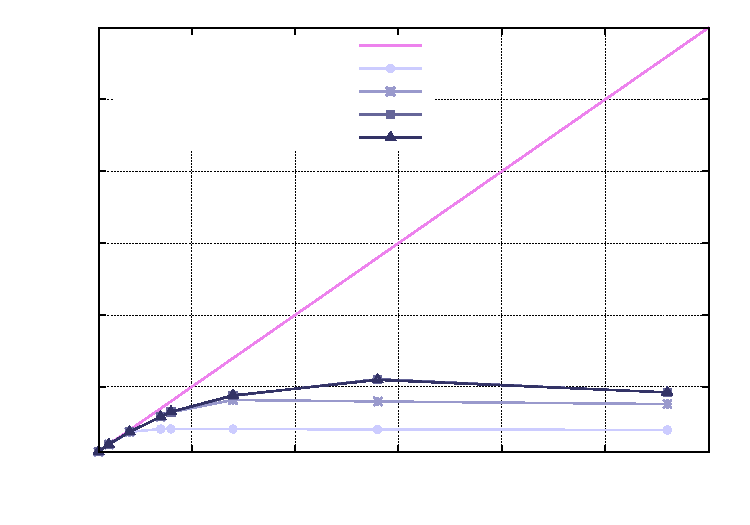
\includegraphics{plot-T-s_nogatherInt_11_500_selected_56}}%
    \gplfronttext
  \end{picture}%
\endgroup
}
      \caption{Scalabilit\`a dell'implementazione SM con M=56 al variare del tempo di interarrivo}
      \label{fig:scalability_SM_size56}
    \end{subfigure}
    ~
    \begin{subfigure}[b]{\textwidth}
      \centering
      \addtocounter{subfigure}{-1}
      \renewcommand\thesubfigure{\alph{subfigure}2}
      \resizebox{\columnwidth}{!}{% GNUPLOT: LaTeX picture with Postscript
\begingroup
  \makeatletter
  \providecommand\color[2][]{%
    \GenericError{(gnuplot) \space\space\space\@spaces}{%
      Package color not loaded in conjunction with
      terminal option `colourtext'%
    }{See the gnuplot documentation for explanation.%
    }{Either use 'blacktext' in gnuplot or load the package
      color.sty in LaTeX.}%
    \renewcommand\color[2][]{}%
  }%
  \providecommand\includegraphics[2][]{%
    \GenericError{(gnuplot) \space\space\space\@spaces}{%
      Package graphicx or graphics not loaded%
    }{See the gnuplot documentation for explanation.%
    }{The gnuplot epslatex terminal needs graphicx.sty or graphics.sty.}%
    \renewcommand\includegraphics[2][]{}%
  }%
  \providecommand\rotatebox[2]{#2}%
  \@ifundefined{ifGPcolor}{%
    \newif\ifGPcolor
    \GPcolortrue
  }{}%
  \@ifundefined{ifGPblacktext}{%
    \newif\ifGPblacktext
    \GPblacktexttrue
  }{}%
  % define a \g@addto@macro without @ in the name:
  \let\gplgaddtomacro\g@addto@macro
  % define empty templates for all commands taking text:
  \gdef\gplbacktext{}%
  \gdef\gplfronttext{}%
  \makeatother
  \ifGPblacktext
    % no textcolor at all
    \def\colorrgb#1{}%
    \def\colorgray#1{}%
  \else
    % gray or color?
    \ifGPcolor
      \def\colorrgb#1{\color[rgb]{#1}}%
      \def\colorgray#1{\color[gray]{#1}}%
      \expandafter\def\csname LTw\endcsname{\color{white}}%
      \expandafter\def\csname LTb\endcsname{\color{black}}%
      \expandafter\def\csname LTa\endcsname{\color{black}}%
      \expandafter\def\csname LT0\endcsname{\color[rgb]{1,0,0}}%
      \expandafter\def\csname LT1\endcsname{\color[rgb]{0,1,0}}%
      \expandafter\def\csname LT2\endcsname{\color[rgb]{0,0,1}}%
      \expandafter\def\csname LT3\endcsname{\color[rgb]{1,0,1}}%
      \expandafter\def\csname LT4\endcsname{\color[rgb]{0,1,1}}%
      \expandafter\def\csname LT5\endcsname{\color[rgb]{1,1,0}}%
      \expandafter\def\csname LT6\endcsname{\color[rgb]{0,0,0}}%
      \expandafter\def\csname LT7\endcsname{\color[rgb]{1,0.3,0}}%
      \expandafter\def\csname LT8\endcsname{\color[rgb]{0.5,0.5,0.5}}%
    \else
      % gray
      \def\colorrgb#1{\color{black}}%
      \def\colorgray#1{\color[gray]{#1}}%
      \expandafter\def\csname LTw\endcsname{\color{white}}%
      \expandafter\def\csname LTb\endcsname{\color{black}}%
      \expandafter\def\csname LTa\endcsname{\color{black}}%
      \expandafter\def\csname LT0\endcsname{\color{black}}%
      \expandafter\def\csname LT1\endcsname{\color{black}}%
      \expandafter\def\csname LT2\endcsname{\color{black}}%
      \expandafter\def\csname LT3\endcsname{\color{black}}%
      \expandafter\def\csname LT4\endcsname{\color{black}}%
      \expandafter\def\csname LT5\endcsname{\color{black}}%
      \expandafter\def\csname LT6\endcsname{\color{black}}%
      \expandafter\def\csname LT7\endcsname{\color{black}}%
      \expandafter\def\csname LT8\endcsname{\color{black}}%
    \fi
  \fi
  \setlength{\unitlength}{0.0500bp}%
  \begin{picture}(7200.00,5040.00)%
    \gplgaddtomacro\gplbacktext{%
      \csname LTb\endcsname%
      \put(814,1325){\makebox(0,0)[r]{\strut{} 10}}%
      \csname LTb\endcsname%
      \put(814,2015){\makebox(0,0)[r]{\strut{} 20}}%
      \csname LTb\endcsname%
      \put(814,2705){\makebox(0,0)[r]{\strut{} 30}}%
      \csname LTb\endcsname%
      \put(814,3395){\makebox(0,0)[r]{\strut{} 40}}%
      \csname LTb\endcsname%
      \put(814,4085){\makebox(0,0)[r]{\strut{} 50}}%
      \csname LTb\endcsname%
      \put(814,4775){\makebox(0,0)[r]{\strut{} 60}}%
      \csname LTb\endcsname%
      \put(1839,484){\makebox(0,0){\strut{} 10}}%
      \csname LTb\endcsname%
      \put(2832,484){\makebox(0,0){\strut{} 20}}%
      \csname LTb\endcsname%
      \put(3825,484){\makebox(0,0){\strut{} 30}}%
      \csname LTb\endcsname%
      \put(4818,484){\makebox(0,0){\strut{} 40}}%
      \csname LTb\endcsname%
      \put(5810,484){\makebox(0,0){\strut{} 50}}%
      \csname LTb\endcsname%
      \put(6803,484){\makebox(0,0){\strut{} 60}}%
      \put(176,2739){\rotatebox{-270}{\makebox(0,0){\strut{}scalability}}}%
      \put(3874,154){\makebox(0,0){\strut{}$n$ parallel degree}}%
    }%
    \gplgaddtomacro\gplfronttext{%
      \csname LTb\endcsname%
      \put(3322,4602){\makebox(0,0)[r]{\strut{}ideal scalability}}%
      \csname LTb\endcsname%
      \put(3322,4382){\makebox(0,0)[r]{\strut{}$T_A$ 150000 $\tau$}}%
      \csname LTb\endcsname%
      \put(3322,4162){\makebox(0,0)[r]{\strut{}$T_A$ 80000 $\tau$}}%
      \csname LTb\endcsname%
      \put(3322,3942){\makebox(0,0)[r]{\strut{}$T_A$ 50000 $\tau$}}%
      \csname LTb\endcsname%
      \put(3322,3722){\makebox(0,0)[r]{\strut{}$T_A$ 35000 $\tau$}}%
      \csname LTb\endcsname%
      \put(3322,3502){\makebox(0,0)[r]{\strut{}$T_A$ 20000 $\tau$}}%
    }%
    \gplbacktext
    \put(0,0){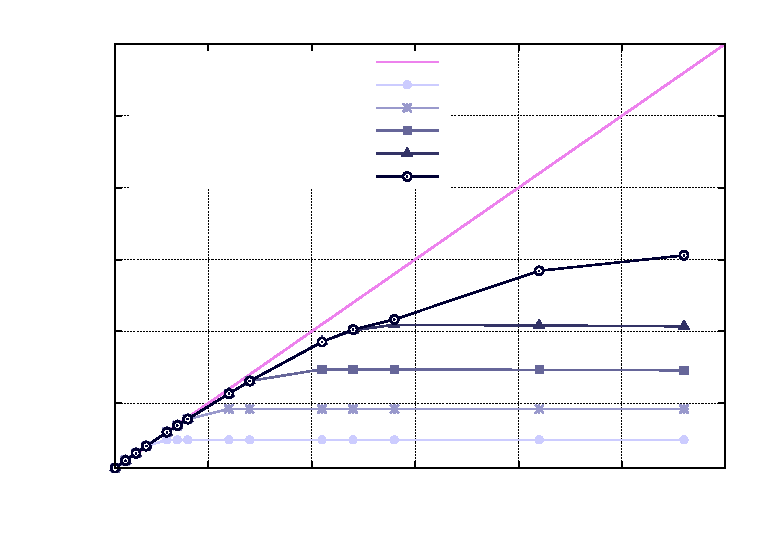
\includegraphics{plot-T-s_nogatherInt_11_500_selected_168}}%
    \gplfronttext
  \end{picture}%
\endgroup
}
      \caption{Scalabilit\`a dell'implementazione SM con M=168 al variare del tempo di interarrivo}
      \label{fig:scalability_SM_size168}
    \end{subfigure}
    ~
    \begin{subfigure}[b]{\textwidth}
      \centering
      \addtocounter{subfigure}{-1}
      \renewcommand\thesubfigure{\alph{subfigure}3}
      \resizebox{\columnwidth}{!}{% GNUPLOT: LaTeX picture with Postscript
\begingroup
  \makeatletter
  \providecommand\color[2][]{%
    \GenericError{(gnuplot) \space\space\space\@spaces}{%
      Package color not loaded in conjunction with
      terminal option `colourtext'%
    }{See the gnuplot documentation for explanation.%
    }{Either use 'blacktext' in gnuplot or load the package
      color.sty in LaTeX.}%
    \renewcommand\color[2][]{}%
  }%
  \providecommand\includegraphics[2][]{%
    \GenericError{(gnuplot) \space\space\space\@spaces}{%
      Package graphicx or graphics not loaded%
    }{See the gnuplot documentation for explanation.%
    }{The gnuplot epslatex terminal needs graphicx.sty or graphics.sty.}%
    \renewcommand\includegraphics[2][]{}%
  }%
  \providecommand\rotatebox[2]{#2}%
  \@ifundefined{ifGPcolor}{%
    \newif\ifGPcolor
    \GPcolortrue
  }{}%
  \@ifundefined{ifGPblacktext}{%
    \newif\ifGPblacktext
    \GPblacktexttrue
  }{}%
  % define a \g@addto@macro without @ in the name:
  \let\gplgaddtomacro\g@addto@macro
  % define empty templates for all commands taking text:
  \gdef\gplbacktext{}%
  \gdef\gplfronttext{}%
  \makeatother
  \ifGPblacktext
    % no textcolor at all
    \def\colorrgb#1{}%
    \def\colorgray#1{}%
  \else
    % gray or color?
    \ifGPcolor
      \def\colorrgb#1{\color[rgb]{#1}}%
      \def\colorgray#1{\color[gray]{#1}}%
      \expandafter\def\csname LTw\endcsname{\color{white}}%
      \expandafter\def\csname LTb\endcsname{\color{black}}%
      \expandafter\def\csname LTa\endcsname{\color{black}}%
      \expandafter\def\csname LT0\endcsname{\color[rgb]{1,0,0}}%
      \expandafter\def\csname LT1\endcsname{\color[rgb]{0,1,0}}%
      \expandafter\def\csname LT2\endcsname{\color[rgb]{0,0,1}}%
      \expandafter\def\csname LT3\endcsname{\color[rgb]{1,0,1}}%
      \expandafter\def\csname LT4\endcsname{\color[rgb]{0,1,1}}%
      \expandafter\def\csname LT5\endcsname{\color[rgb]{1,1,0}}%
      \expandafter\def\csname LT6\endcsname{\color[rgb]{0,0,0}}%
      \expandafter\def\csname LT7\endcsname{\color[rgb]{1,0.3,0}}%
      \expandafter\def\csname LT8\endcsname{\color[rgb]{0.5,0.5,0.5}}%
    \else
      % gray
      \def\colorrgb#1{\color{black}}%
      \def\colorgray#1{\color[gray]{#1}}%
      \expandafter\def\csname LTw\endcsname{\color{white}}%
      \expandafter\def\csname LTb\endcsname{\color{black}}%
      \expandafter\def\csname LTa\endcsname{\color{black}}%
      \expandafter\def\csname LT0\endcsname{\color{black}}%
      \expandafter\def\csname LT1\endcsname{\color{black}}%
      \expandafter\def\csname LT2\endcsname{\color{black}}%
      \expandafter\def\csname LT3\endcsname{\color{black}}%
      \expandafter\def\csname LT4\endcsname{\color{black}}%
      \expandafter\def\csname LT5\endcsname{\color{black}}%
      \expandafter\def\csname LT6\endcsname{\color{black}}%
      \expandafter\def\csname LT7\endcsname{\color{black}}%
      \expandafter\def\csname LT8\endcsname{\color{black}}%
    \fi
  \fi
  \setlength{\unitlength}{0.0500bp}%
  \begin{picture}(7200.00,5040.00)%
    \gplgaddtomacro\gplbacktext{%
      \csname LTb\endcsname%
      \put(814,1325){\makebox(0,0)[r]{\strut{} 10}}%
      \csname LTb\endcsname%
      \put(814,2015){\makebox(0,0)[r]{\strut{} 20}}%
      \csname LTb\endcsname%
      \put(814,2705){\makebox(0,0)[r]{\strut{} 30}}%
      \csname LTb\endcsname%
      \put(814,3395){\makebox(0,0)[r]{\strut{} 40}}%
      \csname LTb\endcsname%
      \put(814,4085){\makebox(0,0)[r]{\strut{} 50}}%
      \csname LTb\endcsname%
      \put(814,4775){\makebox(0,0)[r]{\strut{} 60}}%
      \csname LTb\endcsname%
      \put(1839,484){\makebox(0,0){\strut{} 10}}%
      \csname LTb\endcsname%
      \put(2832,484){\makebox(0,0){\strut{} 20}}%
      \csname LTb\endcsname%
      \put(3825,484){\makebox(0,0){\strut{} 30}}%
      \csname LTb\endcsname%
      \put(4818,484){\makebox(0,0){\strut{} 40}}%
      \csname LTb\endcsname%
      \put(5810,484){\makebox(0,0){\strut{} 50}}%
      \csname LTb\endcsname%
      \put(6803,484){\makebox(0,0){\strut{} 60}}%
      \put(176,2739){\rotatebox{-270}{\makebox(0,0){\strut{}scalability}}}%
      \put(3874,154){\makebox(0,0){\strut{}$n$ parallel degree}}%
    }%
    \gplgaddtomacro\gplfronttext{%
      \csname LTb\endcsname%
      \put(3322,4602){\makebox(0,0)[r]{\strut{}ideal scalability}}%
      \csname LTb\endcsname%
      \put(3322,4382){\makebox(0,0)[r]{\strut{}$T_A$ 250000 $\tau$}}%
      \csname LTb\endcsname%
      \put(3322,4162){\makebox(0,0)[r]{\strut{}$T_A$ 150000 $\tau$}}%
      \csname LTb\endcsname%
      \put(3322,3942){\makebox(0,0)[r]{\strut{}$T_A$ 100000 $\tau$}}%
      \csname LTb\endcsname%
      \put(3322,3722){\makebox(0,0)[r]{\strut{}$T_A$ 80000 $\tau$}}%
      \csname LTb\endcsname%
      \put(3322,3502){\makebox(0,0)[r]{\strut{}$T_A$ 50000 $\tau$}}%
    }%
    \gplbacktext
    \put(0,0){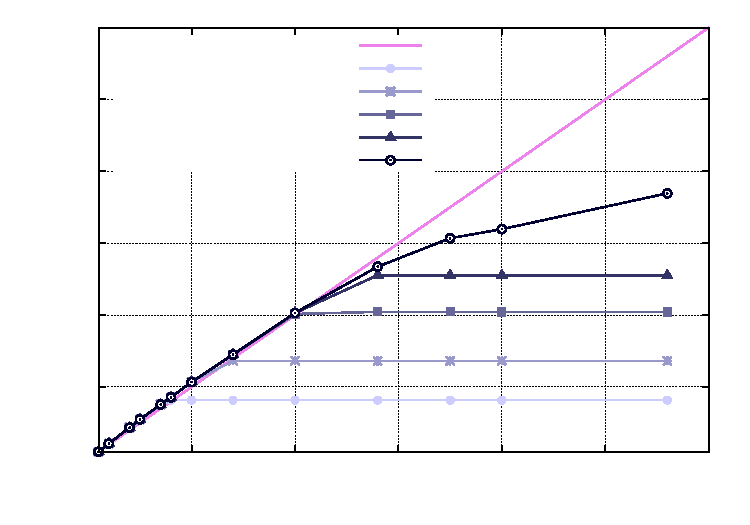
\includegraphics{plot-T-s_nogatherInt_11_500_selected_280}}%
    \gplfronttext
  \end{picture}%
\endgroup
}
      \caption{Scalabilit\`a dell'implementazione SM con M=280 al variare del tempo di interarrivo}
      \label{fig:scalability_SM_size280}
    \end{subfigure}
    \label{fig:allscalability_SM}
  \end{subfigure}
\end{figure}


%%%%%%%%%%%%%%%%%%%%%%%%%%%%%%%%%%%%%%%%%%%%%%%%%%%%%%%%%%%%%%%%%%%%%%%%%%%%%%%%


\begin{figure}[p]
  \caption{Grafici del tempo di servizio al variare del tempo di interarrivo}
  \begin{subfigure}[b]{.5\columnwidth}
    \centering
    \renewcommand\thesubfigure{\alph{subfigure}}
    %% se vuoi spostare questa caption in fondo devi modificare anche i contatori!
    \caption{Implementazione con solo UDN}
    \begin{subfigure}[b]{\textwidth}
      \centering
      \addtocounter{subfigure}{-1}
      \renewcommand\thesubfigure{\alph{subfigure}1}
      \resizebox{\columnwidth}{!}{% GNUPLOT: LaTeX picture with Postscript
\begingroup
  \makeatletter
  \providecommand\color[2][]{%
    \GenericError{(gnuplot) \space\space\space\@spaces}{%
      Package color not loaded in conjunction with
      terminal option `colourtext'%
    }{See the gnuplot documentation for explanation.%
    }{Either use 'blacktext' in gnuplot or load the package
      color.sty in LaTeX.}%
    \renewcommand\color[2][]{}%
  }%
  \providecommand\includegraphics[2][]{%
    \GenericError{(gnuplot) \space\space\space\@spaces}{%
      Package graphicx or graphics not loaded%
    }{See the gnuplot documentation for explanation.%
    }{The gnuplot epslatex terminal needs graphicx.sty or graphics.sty.}%
    \renewcommand\includegraphics[2][]{}%
  }%
  \providecommand\rotatebox[2]{#2}%
  \@ifundefined{ifGPcolor}{%
    \newif\ifGPcolor
    \GPcolortrue
  }{}%
  \@ifundefined{ifGPblacktext}{%
    \newif\ifGPblacktext
    \GPblacktexttrue
  }{}%
  % define a \g@addto@macro without @ in the name:
  \let\gplgaddtomacro\g@addto@macro
  % define empty templates for all commands taking text:
  \gdef\gplbacktext{}%
  \gdef\gplfronttext{}%
  \makeatother
  \ifGPblacktext
    % no textcolor at all
    \def\colorrgb#1{}%
    \def\colorgray#1{}%
  \else
    % gray or color?
    \ifGPcolor
      \def\colorrgb#1{\color[rgb]{#1}}%
      \def\colorgray#1{\color[gray]{#1}}%
      \expandafter\def\csname LTw\endcsname{\color{white}}%
      \expandafter\def\csname LTb\endcsname{\color{black}}%
      \expandafter\def\csname LTa\endcsname{\color{black}}%
      \expandafter\def\csname LT0\endcsname{\color[rgb]{1,0,0}}%
      \expandafter\def\csname LT1\endcsname{\color[rgb]{0,1,0}}%
      \expandafter\def\csname LT2\endcsname{\color[rgb]{0,0,1}}%
      \expandafter\def\csname LT3\endcsname{\color[rgb]{1,0,1}}%
      \expandafter\def\csname LT4\endcsname{\color[rgb]{0,1,1}}%
      \expandafter\def\csname LT5\endcsname{\color[rgb]{1,1,0}}%
      \expandafter\def\csname LT6\endcsname{\color[rgb]{0,0,0}}%
      \expandafter\def\csname LT7\endcsname{\color[rgb]{1,0.3,0}}%
      \expandafter\def\csname LT8\endcsname{\color[rgb]{0.5,0.5,0.5}}%
    \else
      % gray
      \def\colorrgb#1{\color{black}}%
      \def\colorgray#1{\color[gray]{#1}}%
      \expandafter\def\csname LTw\endcsname{\color{white}}%
      \expandafter\def\csname LTb\endcsname{\color{black}}%
      \expandafter\def\csname LTa\endcsname{\color{black}}%
      \expandafter\def\csname LT0\endcsname{\color{black}}%
      \expandafter\def\csname LT1\endcsname{\color{black}}%
      \expandafter\def\csname LT2\endcsname{\color{black}}%
      \expandafter\def\csname LT3\endcsname{\color{black}}%
      \expandafter\def\csname LT4\endcsname{\color{black}}%
      \expandafter\def\csname LT5\endcsname{\color{black}}%
      \expandafter\def\csname LT6\endcsname{\color{black}}%
      \expandafter\def\csname LT7\endcsname{\color{black}}%
      \expandafter\def\csname LT8\endcsname{\color{black}}%
    \fi
  \fi
  \setlength{\unitlength}{0.0500bp}%
  \begin{picture}(7200.00,5040.00)%
    \gplgaddtomacro\gplbacktext{%
      \csname LTb\endcsname%
      \put(1342,704){\makebox(0,0)[r]{\strut{} 1000}}%
      \put(1342,1722){\makebox(0,0)[r]{\strut{} 10000}}%
      \put(1342,2740){\makebox(0,0)[r]{\strut{} 100000}}%
      \put(1342,3757){\makebox(0,0)[r]{\strut{} 1e+06}}%
      \put(1342,4775){\makebox(0,0)[r]{\strut{} 1e+07}}%
      \put(2287,484){\makebox(0,0){\strut{} 10}}%
      \put(3190,484){\makebox(0,0){\strut{} 20}}%
      \put(4093,484){\makebox(0,0){\strut{} 30}}%
      \put(4997,484){\makebox(0,0){\strut{} 40}}%
      \put(5900,484){\makebox(0,0){\strut{} 50}}%
      \put(6803,484){\makebox(0,0){\strut{} 60}}%
      \put(176,2739){\rotatebox{-270}{\makebox(0,0){\strut{}service time ($\tau$)}}}%
      \put(4138,154){\makebox(0,0){\strut{}parallel degree}}%
    }%
    \gplgaddtomacro\gplfronttext{%
      \csname LTb\endcsname%
      \put(2926,4602){\makebox(0,0)[r]{\strut{}$T_A$ 20000 $\tau$}}%
      \csname LTb\endcsname%
      \put(2926,4382){\makebox(0,0)[r]{\strut{}$T_A$ 10000 $\tau$}}%
      \csname LTb\endcsname%
      \put(2926,4162){\makebox(0,0)[r]{\strut{}$T_A$ 7000 $\tau$}}%
      \csname LTb\endcsname%
      \put(2926,3942){\makebox(0,0)[r]{\strut{}$T_A$ 4000 $\tau$}}%
    }%
    \gplbacktext
    \put(0,0){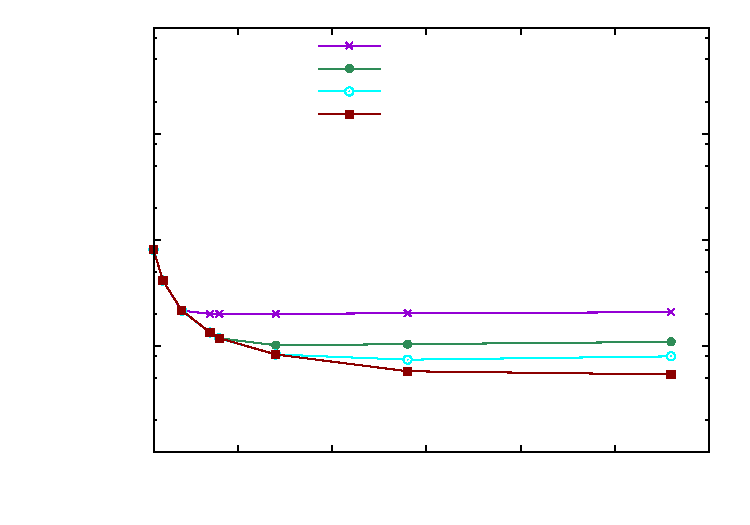
\includegraphics{plot-T_nogatherInt_00_500_selected_56}}%
    \gplfronttext
  \end{picture}%
\endgroup
}
      \caption{Tempo di servizio dell'implementazione UDN con M=56 al variare del tempo di interarrivo}
      \label{fig:scalability_UDN_size56}
    \end{subfigure}
    ~
    \begin{subfigure}[b]{\textwidth}
      \centering
      \addtocounter{subfigure}{-1}
      \renewcommand\thesubfigure{\alph{subfigure}2}
      \resizebox{\columnwidth}{!}{% GNUPLOT: LaTeX picture with Postscript
\begingroup
  \makeatletter
  \providecommand\color[2][]{%
    \GenericError{(gnuplot) \space\space\space\@spaces}{%
      Package color not loaded in conjunction with
      terminal option `colourtext'%
    }{See the gnuplot documentation for explanation.%
    }{Either use 'blacktext' in gnuplot or load the package
      color.sty in LaTeX.}%
    \renewcommand\color[2][]{}%
  }%
  \providecommand\includegraphics[2][]{%
    \GenericError{(gnuplot) \space\space\space\@spaces}{%
      Package graphicx or graphics not loaded%
    }{See the gnuplot documentation for explanation.%
    }{The gnuplot epslatex terminal needs graphicx.sty or graphics.sty.}%
    \renewcommand\includegraphics[2][]{}%
  }%
  \providecommand\rotatebox[2]{#2}%
  \@ifundefined{ifGPcolor}{%
    \newif\ifGPcolor
    \GPcolortrue
  }{}%
  \@ifundefined{ifGPblacktext}{%
    \newif\ifGPblacktext
    \GPblacktexttrue
  }{}%
  % define a \g@addto@macro without @ in the name:
  \let\gplgaddtomacro\g@addto@macro
  % define empty templates for all commands taking text:
  \gdef\gplbacktext{}%
  \gdef\gplfronttext{}%
  \makeatother
  \ifGPblacktext
    % no textcolor at all
    \def\colorrgb#1{}%
    \def\colorgray#1{}%
  \else
    % gray or color?
    \ifGPcolor
      \def\colorrgb#1{\color[rgb]{#1}}%
      \def\colorgray#1{\color[gray]{#1}}%
      \expandafter\def\csname LTw\endcsname{\color{white}}%
      \expandafter\def\csname LTb\endcsname{\color{black}}%
      \expandafter\def\csname LTa\endcsname{\color{black}}%
      \expandafter\def\csname LT0\endcsname{\color[rgb]{1,0,0}}%
      \expandafter\def\csname LT1\endcsname{\color[rgb]{0,1,0}}%
      \expandafter\def\csname LT2\endcsname{\color[rgb]{0,0,1}}%
      \expandafter\def\csname LT3\endcsname{\color[rgb]{1,0,1}}%
      \expandafter\def\csname LT4\endcsname{\color[rgb]{0,1,1}}%
      \expandafter\def\csname LT5\endcsname{\color[rgb]{1,1,0}}%
      \expandafter\def\csname LT6\endcsname{\color[rgb]{0,0,0}}%
      \expandafter\def\csname LT7\endcsname{\color[rgb]{1,0.3,0}}%
      \expandafter\def\csname LT8\endcsname{\color[rgb]{0.5,0.5,0.5}}%
    \else
      % gray
      \def\colorrgb#1{\color{black}}%
      \def\colorgray#1{\color[gray]{#1}}%
      \expandafter\def\csname LTw\endcsname{\color{white}}%
      \expandafter\def\csname LTb\endcsname{\color{black}}%
      \expandafter\def\csname LTa\endcsname{\color{black}}%
      \expandafter\def\csname LT0\endcsname{\color{black}}%
      \expandafter\def\csname LT1\endcsname{\color{black}}%
      \expandafter\def\csname LT2\endcsname{\color{black}}%
      \expandafter\def\csname LT3\endcsname{\color{black}}%
      \expandafter\def\csname LT4\endcsname{\color{black}}%
      \expandafter\def\csname LT5\endcsname{\color{black}}%
      \expandafter\def\csname LT6\endcsname{\color{black}}%
      \expandafter\def\csname LT7\endcsname{\color{black}}%
      \expandafter\def\csname LT8\endcsname{\color{black}}%
    \fi
  \fi
  \setlength{\unitlength}{0.0500bp}%
  \begin{picture}(7200.00,5040.00)%
    \gplgaddtomacro\gplbacktext{%
      \csname LTb\endcsname%
      \put(1342,704){\makebox(0,0)[r]{\strut{} 1000}}%
      \put(1342,1722){\makebox(0,0)[r]{\strut{} 10000}}%
      \put(1342,2740){\makebox(0,0)[r]{\strut{} 100000}}%
      \put(1342,3757){\makebox(0,0)[r]{\strut{} 1e+06}}%
      \put(1342,4775){\makebox(0,0)[r]{\strut{} 1e+07}}%
      \put(2287,484){\makebox(0,0){\strut{} 10}}%
      \put(3190,484){\makebox(0,0){\strut{} 20}}%
      \put(4093,484){\makebox(0,0){\strut{} 30}}%
      \put(4997,484){\makebox(0,0){\strut{} 40}}%
      \put(5900,484){\makebox(0,0){\strut{} 50}}%
      \put(6803,484){\makebox(0,0){\strut{} 60}}%
      \put(176,2739){\rotatebox{-270}{\makebox(0,0){\strut{}service time ($\tau$)}}}%
      \put(4138,154){\makebox(0,0){\strut{}parallel degree}}%
    }%
    \gplgaddtomacro\gplfronttext{%
      \csname LTb\endcsname%
      \put(3058,4602){\makebox(0,0)[r]{\strut{}$T_A$ 150000 $\tau$}}%
      \csname LTb\endcsname%
      \put(3058,4382){\makebox(0,0)[r]{\strut{}$T_A$ 80000 $\tau$}}%
      \csname LTb\endcsname%
      \put(3058,4162){\makebox(0,0)[r]{\strut{}$T_A$ 50000 $\tau$}}%
      \csname LTb\endcsname%
      \put(3058,3942){\makebox(0,0)[r]{\strut{}$T_A$ 35000 $\tau$}}%
      \csname LTb\endcsname%
      \put(3058,3722){\makebox(0,0)[r]{\strut{}$T_A$ 20000 $\tau$}}%
    }%
    \gplbacktext
    \put(0,0){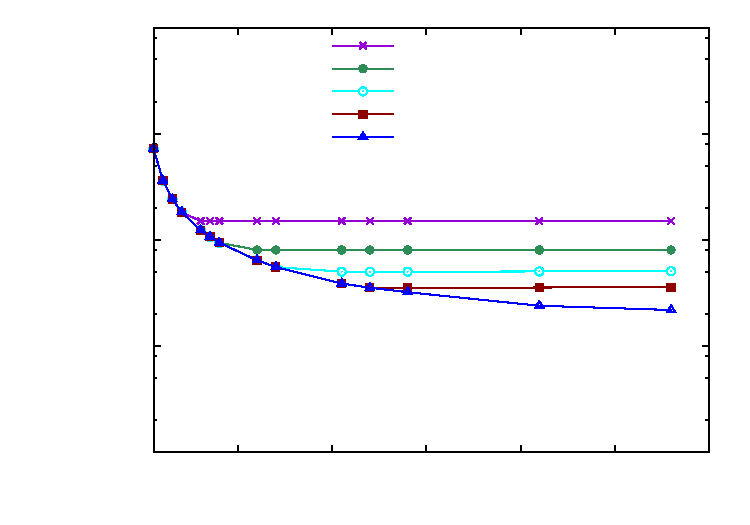
\includegraphics{plot-T_nogatherInt_00_500_selected_168}}%
    \gplfronttext
  \end{picture}%
\endgroup
}
      \caption{Tempo di servizio dell'implementazione UDN con M=168 al variare del tempo di interarrivo}
      \label{fig:scalability_UDN_size168}
    \end{subfigure}
    ~
    \begin{subfigure}[b]{\textwidth}
      \centering
      \addtocounter{subfigure}{-1}
      \renewcommand\thesubfigure{\alph{subfigure}3}
      \resizebox{\columnwidth}{!}{% GNUPLOT: LaTeX picture with Postscript
\begingroup
  \makeatletter
  \providecommand\color[2][]{%
    \GenericError{(gnuplot) \space\space\space\@spaces}{%
      Package color not loaded in conjunction with
      terminal option `colourtext'%
    }{See the gnuplot documentation for explanation.%
    }{Either use 'blacktext' in gnuplot or load the package
      color.sty in LaTeX.}%
    \renewcommand\color[2][]{}%
  }%
  \providecommand\includegraphics[2][]{%
    \GenericError{(gnuplot) \space\space\space\@spaces}{%
      Package graphicx or graphics not loaded%
    }{See the gnuplot documentation for explanation.%
    }{The gnuplot epslatex terminal needs graphicx.sty or graphics.sty.}%
    \renewcommand\includegraphics[2][]{}%
  }%
  \providecommand\rotatebox[2]{#2}%
  \@ifundefined{ifGPcolor}{%
    \newif\ifGPcolor
    \GPcolortrue
  }{}%
  \@ifundefined{ifGPblacktext}{%
    \newif\ifGPblacktext
    \GPblacktexttrue
  }{}%
  % define a \g@addto@macro without @ in the name:
  \let\gplgaddtomacro\g@addto@macro
  % define empty templates for all commands taking text:
  \gdef\gplbacktext{}%
  \gdef\gplfronttext{}%
  \makeatother
  \ifGPblacktext
    % no textcolor at all
    \def\colorrgb#1{}%
    \def\colorgray#1{}%
  \else
    % gray or color?
    \ifGPcolor
      \def\colorrgb#1{\color[rgb]{#1}}%
      \def\colorgray#1{\color[gray]{#1}}%
      \expandafter\def\csname LTw\endcsname{\color{white}}%
      \expandafter\def\csname LTb\endcsname{\color{black}}%
      \expandafter\def\csname LTa\endcsname{\color{black}}%
      \expandafter\def\csname LT0\endcsname{\color[rgb]{1,0,0}}%
      \expandafter\def\csname LT1\endcsname{\color[rgb]{0,1,0}}%
      \expandafter\def\csname LT2\endcsname{\color[rgb]{0,0,1}}%
      \expandafter\def\csname LT3\endcsname{\color[rgb]{1,0,1}}%
      \expandafter\def\csname LT4\endcsname{\color[rgb]{0,1,1}}%
      \expandafter\def\csname LT5\endcsname{\color[rgb]{1,1,0}}%
      \expandafter\def\csname LT6\endcsname{\color[rgb]{0,0,0}}%
      \expandafter\def\csname LT7\endcsname{\color[rgb]{1,0.3,0}}%
      \expandafter\def\csname LT8\endcsname{\color[rgb]{0.5,0.5,0.5}}%
    \else
      % gray
      \def\colorrgb#1{\color{black}}%
      \def\colorgray#1{\color[gray]{#1}}%
      \expandafter\def\csname LTw\endcsname{\color{white}}%
      \expandafter\def\csname LTb\endcsname{\color{black}}%
      \expandafter\def\csname LTa\endcsname{\color{black}}%
      \expandafter\def\csname LT0\endcsname{\color{black}}%
      \expandafter\def\csname LT1\endcsname{\color{black}}%
      \expandafter\def\csname LT2\endcsname{\color{black}}%
      \expandafter\def\csname LT3\endcsname{\color{black}}%
      \expandafter\def\csname LT4\endcsname{\color{black}}%
      \expandafter\def\csname LT5\endcsname{\color{black}}%
      \expandafter\def\csname LT6\endcsname{\color{black}}%
      \expandafter\def\csname LT7\endcsname{\color{black}}%
      \expandafter\def\csname LT8\endcsname{\color{black}}%
    \fi
  \fi
  \setlength{\unitlength}{0.0500bp}%
  \begin{picture}(7200.00,5040.00)%
    \gplgaddtomacro\gplbacktext{%
      \csname LTb\endcsname%
      \put(1342,704){\makebox(0,0)[r]{\strut{} 1000}}%
      \put(1342,1722){\makebox(0,0)[r]{\strut{} 10000}}%
      \put(1342,2740){\makebox(0,0)[r]{\strut{} 100000}}%
      \put(1342,3757){\makebox(0,0)[r]{\strut{} 1e+06}}%
      \put(1342,4775){\makebox(0,0)[r]{\strut{} 1e+07}}%
      \put(2287,484){\makebox(0,0){\strut{} 10}}%
      \put(3190,484){\makebox(0,0){\strut{} 20}}%
      \put(4093,484){\makebox(0,0){\strut{} 30}}%
      \put(4997,484){\makebox(0,0){\strut{} 40}}%
      \put(5900,484){\makebox(0,0){\strut{} 50}}%
      \put(6803,484){\makebox(0,0){\strut{} 60}}%
      \put(176,2739){\rotatebox{-270}{\makebox(0,0){\strut{}service time ($\tau$)}}}%
      \put(4138,154){\makebox(0,0){\strut{}parallel degree}}%
    }%
    \gplgaddtomacro\gplfronttext{%
      \csname LTb\endcsname%
      \put(3058,4602){\makebox(0,0)[r]{\strut{}$T_A$ 250000 $\tau$}}%
      \csname LTb\endcsname%
      \put(3058,4382){\makebox(0,0)[r]{\strut{}$T_A$ 150000 $\tau$}}%
      \csname LTb\endcsname%
      \put(3058,4162){\makebox(0,0)[r]{\strut{}$T_A$ 100000 $\tau$}}%
      \csname LTb\endcsname%
      \put(3058,3942){\makebox(0,0)[r]{\strut{}$T_A$ 80000 $\tau$}}%
      \csname LTb\endcsname%
      \put(3058,3722){\makebox(0,0)[r]{\strut{}$T_A$ 50000 $\tau$}}%
    }%
    \gplbacktext
    \put(0,0){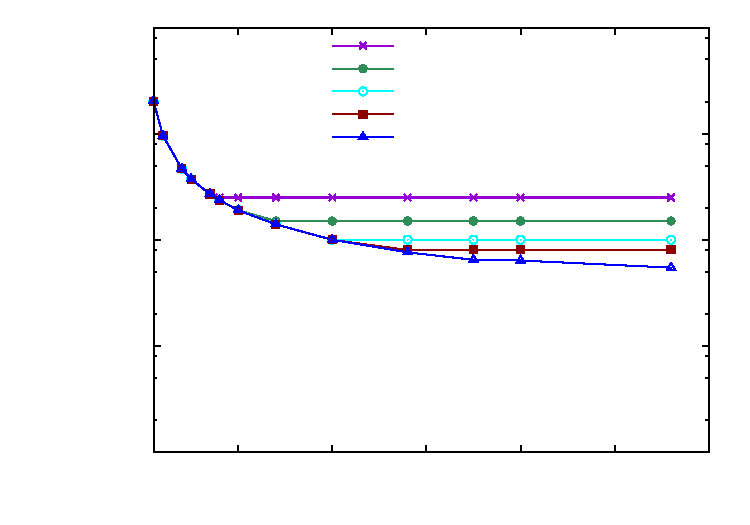
\includegraphics{plot-T_nogatherInt_00_500_selected_280}}%
    \gplfronttext
  \end{picture}%
\endgroup
}
      \caption{Tempo di servizio dell'implementazione UDN con M=280 al variare del tempo di interarrivo}
      \label{fig:scalability_UDN_size280}
    \end{subfigure}
    \label{fig:allScalbility_UDN}
  \end{subfigure}
  \hspace{2ex}
  \begin{subfigure}[b]{.5\columnwidth}
    \centering
    \renewcommand\thesubfigure{\alph{subfigure}}
    \caption{Implementazione con solo SM}
    \begin{subfigure}[b]{\textwidth}
      \centering
      \addtocounter{subfigure}{-1}
      \renewcommand\thesubfigure{\alph{subfigure}1}
      \resizebox{\columnwidth}{!}{% GNUPLOT: LaTeX picture with Postscript
\begingroup
  \makeatletter
  \providecommand\color[2][]{%
    \GenericError{(gnuplot) \space\space\space\@spaces}{%
      Package color not loaded in conjunction with
      terminal option `colourtext'%
    }{See the gnuplot documentation for explanation.%
    }{Either use 'blacktext' in gnuplot or load the package
      color.sty in LaTeX.}%
    \renewcommand\color[2][]{}%
  }%
  \providecommand\includegraphics[2][]{%
    \GenericError{(gnuplot) \space\space\space\@spaces}{%
      Package graphicx or graphics not loaded%
    }{See the gnuplot documentation for explanation.%
    }{The gnuplot epslatex terminal needs graphicx.sty or graphics.sty.}%
    \renewcommand\includegraphics[2][]{}%
  }%
  \providecommand\rotatebox[2]{#2}%
  \@ifundefined{ifGPcolor}{%
    \newif\ifGPcolor
    \GPcolortrue
  }{}%
  \@ifundefined{ifGPblacktext}{%
    \newif\ifGPblacktext
    \GPblacktexttrue
  }{}%
  % define a \g@addto@macro without @ in the name:
  \let\gplgaddtomacro\g@addto@macro
  % define empty templates for all commands taking text:
  \gdef\gplbacktext{}%
  \gdef\gplfronttext{}%
  \makeatother
  \ifGPblacktext
    % no textcolor at all
    \def\colorrgb#1{}%
    \def\colorgray#1{}%
  \else
    % gray or color?
    \ifGPcolor
      \def\colorrgb#1{\color[rgb]{#1}}%
      \def\colorgray#1{\color[gray]{#1}}%
      \expandafter\def\csname LTw\endcsname{\color{white}}%
      \expandafter\def\csname LTb\endcsname{\color{black}}%
      \expandafter\def\csname LTa\endcsname{\color{black}}%
      \expandafter\def\csname LT0\endcsname{\color[rgb]{1,0,0}}%
      \expandafter\def\csname LT1\endcsname{\color[rgb]{0,1,0}}%
      \expandafter\def\csname LT2\endcsname{\color[rgb]{0,0,1}}%
      \expandafter\def\csname LT3\endcsname{\color[rgb]{1,0,1}}%
      \expandafter\def\csname LT4\endcsname{\color[rgb]{0,1,1}}%
      \expandafter\def\csname LT5\endcsname{\color[rgb]{1,1,0}}%
      \expandafter\def\csname LT6\endcsname{\color[rgb]{0,0,0}}%
      \expandafter\def\csname LT7\endcsname{\color[rgb]{1,0.3,0}}%
      \expandafter\def\csname LT8\endcsname{\color[rgb]{0.5,0.5,0.5}}%
    \else
      % gray
      \def\colorrgb#1{\color{black}}%
      \def\colorgray#1{\color[gray]{#1}}%
      \expandafter\def\csname LTw\endcsname{\color{white}}%
      \expandafter\def\csname LTb\endcsname{\color{black}}%
      \expandafter\def\csname LTa\endcsname{\color{black}}%
      \expandafter\def\csname LT0\endcsname{\color{black}}%
      \expandafter\def\csname LT1\endcsname{\color{black}}%
      \expandafter\def\csname LT2\endcsname{\color{black}}%
      \expandafter\def\csname LT3\endcsname{\color{black}}%
      \expandafter\def\csname LT4\endcsname{\color{black}}%
      \expandafter\def\csname LT5\endcsname{\color{black}}%
      \expandafter\def\csname LT6\endcsname{\color{black}}%
      \expandafter\def\csname LT7\endcsname{\color{black}}%
      \expandafter\def\csname LT8\endcsname{\color{black}}%
    \fi
  \fi
  \setlength{\unitlength}{0.0500bp}%
  \begin{picture}(7200.00,5040.00)%
    \gplgaddtomacro\gplbacktext{%
      \csname LTb\endcsname%
      \put(1342,704){\makebox(0,0)[r]{\strut{} 1000}}%
      \put(1342,1722){\makebox(0,0)[r]{\strut{} 10000}}%
      \put(1342,2740){\makebox(0,0)[r]{\strut{} 100000}}%
      \put(1342,3757){\makebox(0,0)[r]{\strut{} 1e+06}}%
      \put(1342,4775){\makebox(0,0)[r]{\strut{} 1e+07}}%
      \put(2287,484){\makebox(0,0){\strut{} 10}}%
      \put(3190,484){\makebox(0,0){\strut{} 20}}%
      \put(4093,484){\makebox(0,0){\strut{} 30}}%
      \put(4997,484){\makebox(0,0){\strut{} 40}}%
      \put(5900,484){\makebox(0,0){\strut{} 50}}%
      \put(6803,484){\makebox(0,0){\strut{} 60}}%
      \put(176,2739){\rotatebox{-270}{\makebox(0,0){\strut{}service time ($\tau$)}}}%
      \put(4138,154){\makebox(0,0){\strut{}parallel degree}}%
    }%
    \gplgaddtomacro\gplfronttext{%
      \csname LTb\endcsname%
      \put(2926,4602){\makebox(0,0)[r]{\strut{}$T_A$ 20000 $\tau$}}%
      \csname LTb\endcsname%
      \put(2926,4382){\makebox(0,0)[r]{\strut{}$T_A$ 10000 $\tau$}}%
      \csname LTb\endcsname%
      \put(2926,4162){\makebox(0,0)[r]{\strut{}$T_A$ 7000 $\tau$}}%
      \csname LTb\endcsname%
      \put(2926,3942){\makebox(0,0)[r]{\strut{}$T_A$ 4000 $\tau$}}%
    }%
    \gplbacktext
    \put(0,0){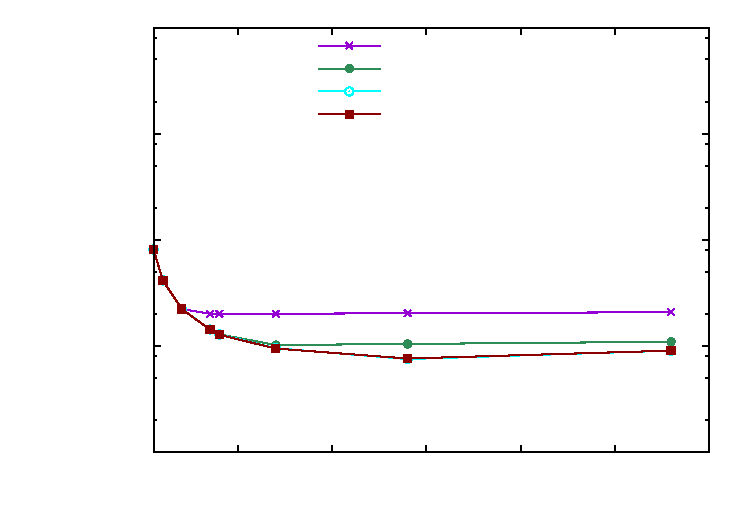
\includegraphics{plot-T_nogatherInt_11_500_selected_56}}%
    \gplfronttext
  \end{picture}%
\endgroup
}
      \caption{Tempo di servizio dell'implementazione SM con M=56 al variare del tempo di interarrivo}
      \label{fig:scalability_SM_size56}
    \end{subfigure}
    ~
    \begin{subfigure}[b]{\textwidth}
      \centering
      \addtocounter{subfigure}{-1}
      \renewcommand\thesubfigure{\alph{subfigure}2}
      \resizebox{\columnwidth}{!}{% GNUPLOT: LaTeX picture with Postscript
\begingroup
  \makeatletter
  \providecommand\color[2][]{%
    \GenericError{(gnuplot) \space\space\space\@spaces}{%
      Package color not loaded in conjunction with
      terminal option `colourtext'%
    }{See the gnuplot documentation for explanation.%
    }{Either use 'blacktext' in gnuplot or load the package
      color.sty in LaTeX.}%
    \renewcommand\color[2][]{}%
  }%
  \providecommand\includegraphics[2][]{%
    \GenericError{(gnuplot) \space\space\space\@spaces}{%
      Package graphicx or graphics not loaded%
    }{See the gnuplot documentation for explanation.%
    }{The gnuplot epslatex terminal needs graphicx.sty or graphics.sty.}%
    \renewcommand\includegraphics[2][]{}%
  }%
  \providecommand\rotatebox[2]{#2}%
  \@ifundefined{ifGPcolor}{%
    \newif\ifGPcolor
    \GPcolortrue
  }{}%
  \@ifundefined{ifGPblacktext}{%
    \newif\ifGPblacktext
    \GPblacktexttrue
  }{}%
  % define a \g@addto@macro without @ in the name:
  \let\gplgaddtomacro\g@addto@macro
  % define empty templates for all commands taking text:
  \gdef\gplbacktext{}%
  \gdef\gplfronttext{}%
  \makeatother
  \ifGPblacktext
    % no textcolor at all
    \def\colorrgb#1{}%
    \def\colorgray#1{}%
  \else
    % gray or color?
    \ifGPcolor
      \def\colorrgb#1{\color[rgb]{#1}}%
      \def\colorgray#1{\color[gray]{#1}}%
      \expandafter\def\csname LTw\endcsname{\color{white}}%
      \expandafter\def\csname LTb\endcsname{\color{black}}%
      \expandafter\def\csname LTa\endcsname{\color{black}}%
      \expandafter\def\csname LT0\endcsname{\color[rgb]{1,0,0}}%
      \expandafter\def\csname LT1\endcsname{\color[rgb]{0,1,0}}%
      \expandafter\def\csname LT2\endcsname{\color[rgb]{0,0,1}}%
      \expandafter\def\csname LT3\endcsname{\color[rgb]{1,0,1}}%
      \expandafter\def\csname LT4\endcsname{\color[rgb]{0,1,1}}%
      \expandafter\def\csname LT5\endcsname{\color[rgb]{1,1,0}}%
      \expandafter\def\csname LT6\endcsname{\color[rgb]{0,0,0}}%
      \expandafter\def\csname LT7\endcsname{\color[rgb]{1,0.3,0}}%
      \expandafter\def\csname LT8\endcsname{\color[rgb]{0.5,0.5,0.5}}%
    \else
      % gray
      \def\colorrgb#1{\color{black}}%
      \def\colorgray#1{\color[gray]{#1}}%
      \expandafter\def\csname LTw\endcsname{\color{white}}%
      \expandafter\def\csname LTb\endcsname{\color{black}}%
      \expandafter\def\csname LTa\endcsname{\color{black}}%
      \expandafter\def\csname LT0\endcsname{\color{black}}%
      \expandafter\def\csname LT1\endcsname{\color{black}}%
      \expandafter\def\csname LT2\endcsname{\color{black}}%
      \expandafter\def\csname LT3\endcsname{\color{black}}%
      \expandafter\def\csname LT4\endcsname{\color{black}}%
      \expandafter\def\csname LT5\endcsname{\color{black}}%
      \expandafter\def\csname LT6\endcsname{\color{black}}%
      \expandafter\def\csname LT7\endcsname{\color{black}}%
      \expandafter\def\csname LT8\endcsname{\color{black}}%
    \fi
  \fi
  \setlength{\unitlength}{0.0500bp}%
  \begin{picture}(7200.00,5040.00)%
    \gplgaddtomacro\gplbacktext{%
      \csname LTb\endcsname%
      \put(1342,704){\makebox(0,0)[r]{\strut{} 1000}}%
      \put(1342,1722){\makebox(0,0)[r]{\strut{} 10000}}%
      \put(1342,2740){\makebox(0,0)[r]{\strut{} 100000}}%
      \put(1342,3757){\makebox(0,0)[r]{\strut{} 1e+06}}%
      \put(1342,4775){\makebox(0,0)[r]{\strut{} 1e+07}}%
      \put(2287,484){\makebox(0,0){\strut{} 10}}%
      \put(3190,484){\makebox(0,0){\strut{} 20}}%
      \put(4093,484){\makebox(0,0){\strut{} 30}}%
      \put(4997,484){\makebox(0,0){\strut{} 40}}%
      \put(5900,484){\makebox(0,0){\strut{} 50}}%
      \put(6803,484){\makebox(0,0){\strut{} 60}}%
      \put(176,2739){\rotatebox{-270}{\makebox(0,0){\strut{}service time ($\tau$)}}}%
      \put(4138,154){\makebox(0,0){\strut{}parallel degree}}%
    }%
    \gplgaddtomacro\gplfronttext{%
      \csname LTb\endcsname%
      \put(3058,4602){\makebox(0,0)[r]{\strut{}$T_A$ 150000 $\tau$}}%
      \csname LTb\endcsname%
      \put(3058,4382){\makebox(0,0)[r]{\strut{}$T_A$ 80000 $\tau$}}%
      \csname LTb\endcsname%
      \put(3058,4162){\makebox(0,0)[r]{\strut{}$T_A$ 50000 $\tau$}}%
      \csname LTb\endcsname%
      \put(3058,3942){\makebox(0,0)[r]{\strut{}$T_A$ 35000 $\tau$}}%
      \csname LTb\endcsname%
      \put(3058,3722){\makebox(0,0)[r]{\strut{}$T_A$ 20000 $\tau$}}%
    }%
    \gplbacktext
    \put(0,0){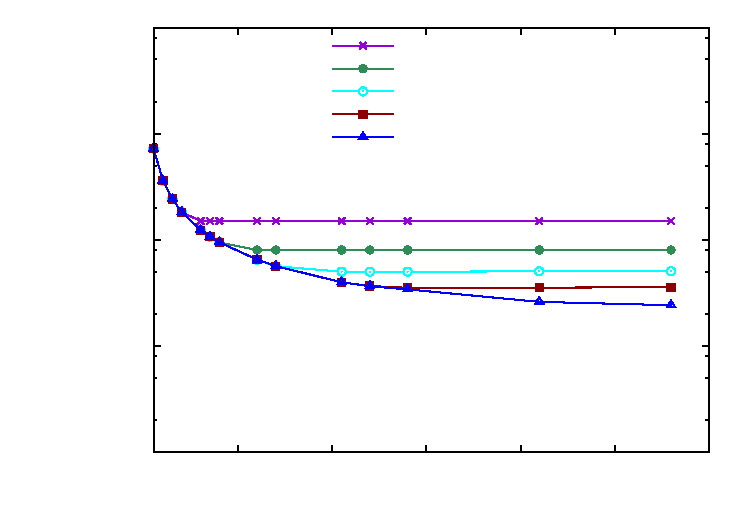
\includegraphics{plot-T_nogatherInt_11_500_selected_168}}%
    \gplfronttext
  \end{picture}%
\endgroup
}
      \caption{Tempo di servizio dell'implementazione SM con M=168 al variare del tempo di interarrivo}
      \label{fig:scalability_SM_size168}
    \end{subfigure}
    ~
    \begin{subfigure}[b]{\textwidth}
      \centering
      \addtocounter{subfigure}{-1}
      \renewcommand\thesubfigure{\alph{subfigure}3}
      \resizebox{\columnwidth}{!}{% GNUPLOT: LaTeX picture with Postscript
\begingroup
  \makeatletter
  \providecommand\color[2][]{%
    \GenericError{(gnuplot) \space\space\space\@spaces}{%
      Package color not loaded in conjunction with
      terminal option `colourtext'%
    }{See the gnuplot documentation for explanation.%
    }{Either use 'blacktext' in gnuplot or load the package
      color.sty in LaTeX.}%
    \renewcommand\color[2][]{}%
  }%
  \providecommand\includegraphics[2][]{%
    \GenericError{(gnuplot) \space\space\space\@spaces}{%
      Package graphicx or graphics not loaded%
    }{See the gnuplot documentation for explanation.%
    }{The gnuplot epslatex terminal needs graphicx.sty or graphics.sty.}%
    \renewcommand\includegraphics[2][]{}%
  }%
  \providecommand\rotatebox[2]{#2}%
  \@ifundefined{ifGPcolor}{%
    \newif\ifGPcolor
    \GPcolortrue
  }{}%
  \@ifundefined{ifGPblacktext}{%
    \newif\ifGPblacktext
    \GPblacktexttrue
  }{}%
  % define a \g@addto@macro without @ in the name:
  \let\gplgaddtomacro\g@addto@macro
  % define empty templates for all commands taking text:
  \gdef\gplbacktext{}%
  \gdef\gplfronttext{}%
  \makeatother
  \ifGPblacktext
    % no textcolor at all
    \def\colorrgb#1{}%
    \def\colorgray#1{}%
  \else
    % gray or color?
    \ifGPcolor
      \def\colorrgb#1{\color[rgb]{#1}}%
      \def\colorgray#1{\color[gray]{#1}}%
      \expandafter\def\csname LTw\endcsname{\color{white}}%
      \expandafter\def\csname LTb\endcsname{\color{black}}%
      \expandafter\def\csname LTa\endcsname{\color{black}}%
      \expandafter\def\csname LT0\endcsname{\color[rgb]{1,0,0}}%
      \expandafter\def\csname LT1\endcsname{\color[rgb]{0,1,0}}%
      \expandafter\def\csname LT2\endcsname{\color[rgb]{0,0,1}}%
      \expandafter\def\csname LT3\endcsname{\color[rgb]{1,0,1}}%
      \expandafter\def\csname LT4\endcsname{\color[rgb]{0,1,1}}%
      \expandafter\def\csname LT5\endcsname{\color[rgb]{1,1,0}}%
      \expandafter\def\csname LT6\endcsname{\color[rgb]{0,0,0}}%
      \expandafter\def\csname LT7\endcsname{\color[rgb]{1,0.3,0}}%
      \expandafter\def\csname LT8\endcsname{\color[rgb]{0.5,0.5,0.5}}%
    \else
      % gray
      \def\colorrgb#1{\color{black}}%
      \def\colorgray#1{\color[gray]{#1}}%
      \expandafter\def\csname LTw\endcsname{\color{white}}%
      \expandafter\def\csname LTb\endcsname{\color{black}}%
      \expandafter\def\csname LTa\endcsname{\color{black}}%
      \expandafter\def\csname LT0\endcsname{\color{black}}%
      \expandafter\def\csname LT1\endcsname{\color{black}}%
      \expandafter\def\csname LT2\endcsname{\color{black}}%
      \expandafter\def\csname LT3\endcsname{\color{black}}%
      \expandafter\def\csname LT4\endcsname{\color{black}}%
      \expandafter\def\csname LT5\endcsname{\color{black}}%
      \expandafter\def\csname LT6\endcsname{\color{black}}%
      \expandafter\def\csname LT7\endcsname{\color{black}}%
      \expandafter\def\csname LT8\endcsname{\color{black}}%
    \fi
  \fi
  \setlength{\unitlength}{0.0500bp}%
  \begin{picture}(7200.00,5040.00)%
    \gplgaddtomacro\gplbacktext{%
      \csname LTb\endcsname%
      \put(1342,704){\makebox(0,0)[r]{\strut{} 1000}}%
      \put(1342,1722){\makebox(0,0)[r]{\strut{} 10000}}%
      \put(1342,2740){\makebox(0,0)[r]{\strut{} 100000}}%
      \put(1342,3757){\makebox(0,0)[r]{\strut{} 1e+06}}%
      \put(1342,4775){\makebox(0,0)[r]{\strut{} 1e+07}}%
      \put(2287,484){\makebox(0,0){\strut{} 10}}%
      \put(3190,484){\makebox(0,0){\strut{} 20}}%
      \put(4093,484){\makebox(0,0){\strut{} 30}}%
      \put(4997,484){\makebox(0,0){\strut{} 40}}%
      \put(5900,484){\makebox(0,0){\strut{} 50}}%
      \put(6803,484){\makebox(0,0){\strut{} 60}}%
      \put(176,2739){\rotatebox{-270}{\makebox(0,0){\strut{}service time ($\tau$)}}}%
      \put(4138,154){\makebox(0,0){\strut{}parallel degree}}%
    }%
    \gplgaddtomacro\gplfronttext{%
      \csname LTb\endcsname%
      \put(3058,4602){\makebox(0,0)[r]{\strut{}$T_A$ 250000 $\tau$}}%
      \csname LTb\endcsname%
      \put(3058,4382){\makebox(0,0)[r]{\strut{}$T_A$ 150000 $\tau$}}%
      \csname LTb\endcsname%
      \put(3058,4162){\makebox(0,0)[r]{\strut{}$T_A$ 100000 $\tau$}}%
      \csname LTb\endcsname%
      \put(3058,3942){\makebox(0,0)[r]{\strut{}$T_A$ 80000 $\tau$}}%
      \csname LTb\endcsname%
      \put(3058,3722){\makebox(0,0)[r]{\strut{}$T_A$ 50000 $\tau$}}%
    }%
    \gplbacktext
    \put(0,0){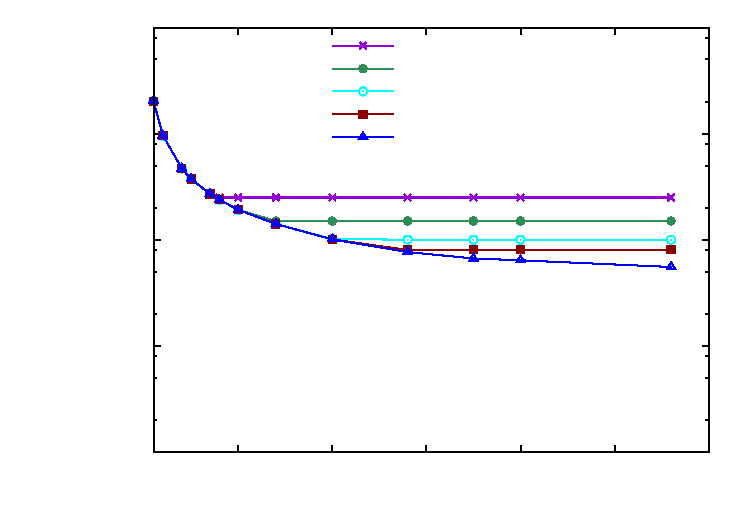
\includegraphics{plot-T_nogatherInt_11_500_selected_280}}%
    \gplfronttext
  \end{picture}%
\endgroup
}
      \caption{Tempo di servizio dell'implementazione SM con M=280 al variare del tempo di interarrivo}
      \label{fig:scalability_SM_size280}
    \end{subfigure}
    \label{fig:allscalability_SM}
  \end{subfigure}
\end{figure}


%%%%%%%%%%%%%%%%%%%%%%%%%%%%%%%%%%%%%%%%%%%%%%%%%%%%%%%%%%%%%%%%%%%%%%%%%%%%%%%%


